% This is samplepaper.tex, a sample chapter demonstrating the
% LLNCS macro package for Springer Computer Science proceedings;
% Version 2.20 of 2017/10/04
%
\documentclass[runningheads]{llncs}
%
\usepackage{graphicx}
% Used for displaying a sample figure. If possible, figure files should
% be included in EPS format.
%
% If you use the hyperref package, please uncomment the following line
% to display URLs in blue roman font according to Springer's eBook style:
%  \renewcommand\UrlFont{\color{blue}\rmfamily}

\begin{document}
%
\title{QALD-Mini-Project}
%
%\titlerunning{Abbreviated paper title}
% If the paper title is too long for the running head, you can set
% an abbreviated paper title here
%
\author{Lukas Bl{\"u}baum \and
Nick D{\"u}sterhus \and
Ralf Keller}
%
\authorrunning{L. Bl{\"u}baum, N. D{\"u}sterhus et al.}
% First names are abbreviated in the running head.
% If there are more than two authors, 'et al.' is used.
%
\institute{University of Paderborn ,Warburger Str. 100, 33098 Paderborn, Germany
\email{\{lukasbl,nduester,rkeller\}@uni-paderborn.de}}

%
\maketitle              % typeset the header of the contribution
%
\begin{abstract}
The abstract should briefly summarize the contents of the paper in
150--250 words.

\keywords{First keyword  \and Second keyword \and Another keyword.}
\end{abstract}
%
%
%
\section{Introduction (Ralf)}  

The World Wide Web is filled with information for everyone to explore. Most information on the Web is unstructured, what makes it hard to process for humans and computers. The Semantic Web is a approach to provide structured data in the Web that is easy to process by computers and can be processed to be easily understood by humans. \\

Most Semantic Web Databases use SPARQL as the language to query the database. That means that in order to search the semantic web the user has to learn a query language, that is not very easy to learn. This is not user friendly and can be improved. \\

The goal of our project is to provide a interface that takes a question formulated in natural language and answers it by querying DBPedia. The interface will be able to be used over the web via HTTP-POST requests. We aim for a F-measure of at last 0.1. \\

Our project uses a Template-based approach. That means we have defined templates of SPARQL-Queries that are modified at predefined locations based on the question asked. The project consists of three components: The \emph{Question-Answering (QA) Engine}, the \emph{Question-Processor} and the \emph{SPARQLQueryBuilder}. We use the Library \emph{qa.annotation} to find entities, propierties and classes, qa.commons to load and store QALD-datasets and GERBIL QA, a wrapper for web communication.   \\

The \emph{QA Engine} is responsible for providing the interface to users. It reads questions from the Webservice or a predefined dataset and passes the question to the Question Processor. Furthermore the QA Engine is responsible for outputting the answer, i.e sending a HTTP-Response to the user. \\

Relevant entities contained in the question have to be identified and the question has to be analyzed to determine the type of the question. This is done by the \emph{Question Processor} component. \\

To get a answer a SPARQL-Query has to be build and executed on a endpoint. That is the responsibility of the \emph{SPARQLQueryBuilder}. This component uses the processed information provided by the Question Processor, builds a SPARQL-Query by using predefined templates and executes the query on an endpoint provided by DBPedia. 

\pagebreak
\section{Simplified Procedure} (Nick)
\begin{figure}
	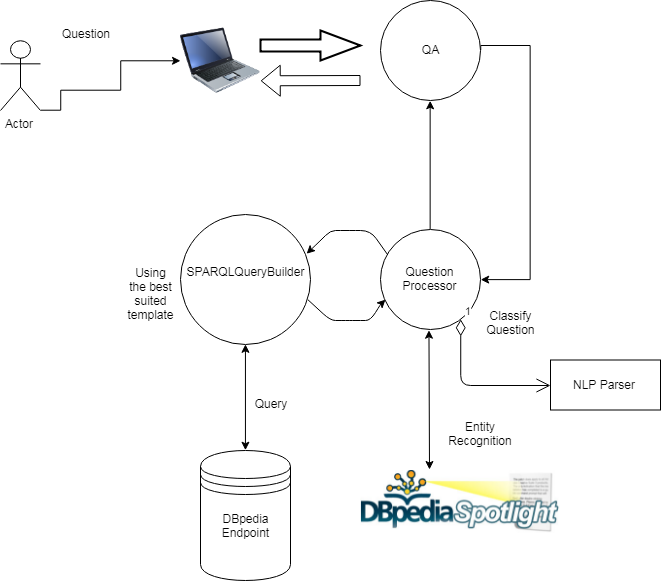
\includegraphics[width=\textwidth]{Architecture.PNG}
	
	\caption{Architecture.}
	\label{fig1} 
\end{figure}

\section{QA System} (Ralf)

\begin{itemize}

	\item Responsible for fetching questions and relaying them to the Question Processor
		\begin{itemize}
			\item Load datasets
			\item Webservice
			\item Single compile-time question
		\end{itemize}

	\item Consists of two subcomponents
		\begin{itemize}
			\item QA
			\item QA-System
		\end{itemize}

	\item QA
		\begin{itemize}
			\item Checks the configured mode 
				\begin{itemize}
					\item Can only be set at compiletime
				\end{itemize}
			\item Relays question or starts webservice, depending on mode
			\item writes answers to JSON-File if mode==dataset
		\end{itemize}

	\item QA-System
		\begin{itemize}
			\item Takes a question and the language of the question
			\item Returns answer container
		\end{itemize}

	\item Answer container
		\begin{itemize}
			\item Contains relevant data for the answer
			\item The answer
			\item the SPARQL-Query used
		\end{itemize}
		
	
\end{itemize}

\subsection{Webservice}

\begin{itemize}
	\item Uses Spring
	\item listens on /gerbil for HTTP-POST requests
	\item reads the question and relays it to the QA-System
	\item returns the result to the sender of the requests as JSON 
\end{itemize}

\section{Question Preprocessing} (Lukas)

\section{Template Overview} (Lukas)

\subsection{Example}

\subsection{Superlatives, Comparatives and Temporal Aggregators} (Ralf) )(Lukas)

\begin{itemize}
	\item predefined enum with comperatives and Superlatives
	\item used to determine the corresponding DBPedia property and sort order
\end{itemize}

\subsection{Example}

\section{Benchmarking and Evaluation} (Nick)

\section{Summary} (Nick)

\begin{figure}
	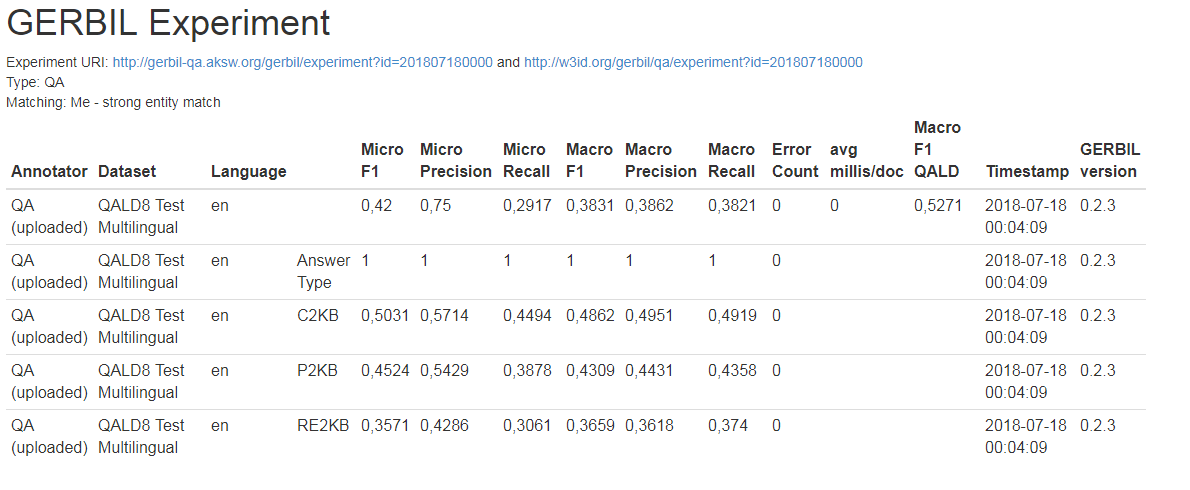
\includegraphics[width=\textwidth]{QALD-8-Test.PNG}
	
	\caption{Gerbil experiment for the QALD8-Test set, with an F-measure of 0.33.}
	 \label{fig2} 
\end{figure}

\subsection{A Subsection Sample}
Please note that the first paragraph of a section or subsection is
not indented. The first paragraph that follows a table, figure,
equation etc. does not need an indent, either.

Subsequent paragraphs, however, are indented.

\subsubsection{Sample Heading (Third Level)} Only two levels of
headings should be numbered. Lower level headings remain unnumbered;
they are formatted as run-in headings.

\paragraph{Sample Heading (Fourth Level)}
The contribution should contain no more than four levels of
headings. Table~\ref{tab1} gives a summary of all heading levels.

\begin{table}
\caption{Table captions should be placed above the
tables.}\label{tab1}
\begin{tabular}{|l|l|l|}
\hline
Heading level &  Example & Font size and style\\
\hline
Title (centered) &  {\Large\bfseries Lecture Notes} & 14 point, bold\\
1st-level heading &  {\large\bfseries 1 Introduction} & 12 point, bold\\
2nd-level heading & {\bfseries 2.1 Printing Area} & 10 point, bold\\
3rd-level heading & {\bfseries Run-in Heading in Bold.} Text follows & 10 point, bold\\
4th-level heading & {\itshape Lowest Level Heading.} Text follows & 10 point, italic\\
\hline
\end{tabular}
\end{table}


\noindent Displayed equations are centered and set on a separate
line.
\begin{equation}
x + y = z
\end{equation}
Please try to avoid rasterized images for line-art diagrams and
schemas. Whenever possible, use vector graphics instead (see
Fig.~\ref{fig3}).

\begin{figure}
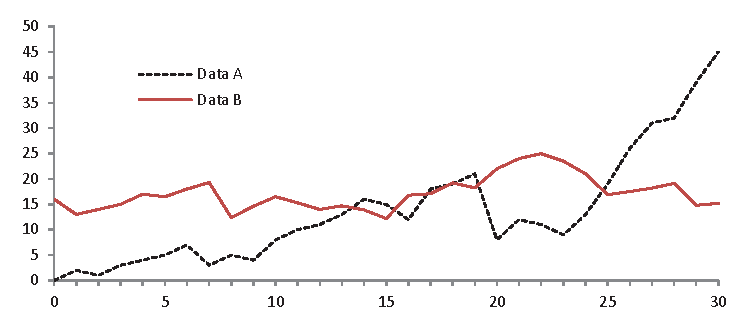
\includegraphics[width=\textwidth]{fig1.eps}
\caption{A figure caption is always placed below the illustration.
Please note that short captions are centered, while long ones are
justified by the macro package automatically.} \label{fig1}
\end{figure}

\begin{theorem}
This is a sample theorem. The run-in heading is set in bold, while
the following text appears in italics. Definitions, lemmas,
propositions, and corollaries are styled the same way.
\end{theorem}
%
% the environments 'definition', 'lemma', 'proposition', 'corollary',
% 'remark', and 'example' are defined in the LLNCS documentclass as well.
%
\begin{proof}
Proofs, examples, and remarks have the initial word in italics,
while the following text appears in normal font.
\end{proof}
For citations of references, we prefer the use of square brackets
and consecutive numbers. Citations using labels or the author/year
convention are also acceptable. The following bibliography provides
a sample reference list with entries for journal
articles~\cite{ref_article1}, an LNCS chapter~\cite{ref_lncs1}, a
book~\cite{ref_book1}, proceedings without editors~\cite{ref_proc1},
and a homepage~\cite{ref_url1}. Multiple citations are grouped
\cite{ref_article1,ref_lncs1,ref_book1},
\cite{ref_article1,ref_book1,ref_proc1,ref_url1}.
%
% ---- Bibliography ----
%
% BibTeX users should specify bibliography style 'splncs04'.
% References will then be sorted and formatted in the correct style.
%
% \bibliographystyle{splncs04}
% \bibliography{mybibliography}
%
\begin{thebibliography}{8}
\bibitem{ref_article1}
Author, F.: Article title. Journal \textbf{2}(5), 99--110 (2016)

\bibitem{ref_lncs1}
Author, F., Author, S.: Title of a proceedings paper. In: Editor,
F., Editor, S. (eds.) CONFERENCE 2016, LNCS, vol. 9999, pp. 1--13.
Springer, Heidelberg (2016). \doi{10.10007/1234567890}

\bibitem{ref_book1}
Author, F., Author, S., Author, T.: Book title. 2nd edn. Publisher,
Location (1999)

\bibitem{ref_proc1}
Author, A.-B.: Contribution title. In: 9th International Proceedings
on Proceedings, pp. 1--2. Publisher, Location (2010)

\bibitem{ref_url1}
LNCS Homepage, \url{http://www.springer.com/lncs}. Last accessed 4
Oct 2017
\end{thebibliography}
\end{document}
